\documentclass[border=-10mm]{standalone}
\usepackage{pgfplots}
\usepackage{tikz}

\begin{document}

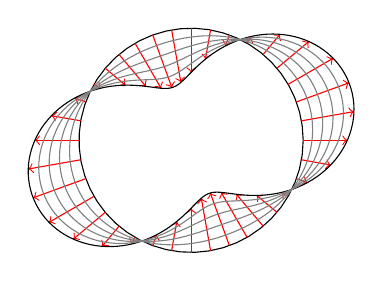
\begin{tikzpicture}
  \begin{axis}[axis lines=none, axis equal,
    xmin=-2,xmax=2,
    ymin=-2,ymax=2,
    samples=200
    ]
    \addplot[domain=0:360,samples=50]
    ({cos(x)},{sin(x)});

    \foreach \q in {1,...,36}
    \addplot[->, red, domain=0:1]
    ({(1+sin((\q *10 + 26)*2)/2*x)*cos(\q *10)},{(1+sin((\q *10 + 26)*2)/2*x)*sin(\q *10)});

    \addplot[black, domain=0:36]
    ({(1+sin((x *10 + 26)*2)/2*1)*cos(x *10)},{(1+sin((x *10 +
      26)*2)/2*1)*sin(x *10)});

    \foreach \t in {1,...,4}
    \addplot[gray, domain=0:36]
    ({(1+sin((x *10 + 26)*2)/2* \t /5)*cos(x *10)},{(1+sin((x *10 +
      26)*2)/2* \t /5)*sin(x *10)});
  \end{axis}
\end{tikzpicture}

\end{document}


